\documentclass[10pt]{beamer}

\usetheme{metropolis}
\usepackage{appendixnumberbeamer}

\usepackage{booktabs}
\usepackage[scale=2]{ccicons}

\usepackage{pgfplots}
\usepgfplotslibrary{dateplot}

\usepackage{xspace}
\newcommand{\themename}{\textbf{\textsc{metropolis}}\xspace}

\usepackage{subfig}
\usepackage{natbib}

\usepackage[
  mathrm=sym,
  % math-style=ISO,  % Greek letters also in italics
  bold-style=ISO,  % bold letters also in italics
]{unicode-math}

% \setmathfont{Fira Math}

\title{3D Reconstruction with Fast Dipole Sums}
\subtitle{MS Thesis Presentation}
\date{April 29, 2024}
\author{Hanyu Chen}
\institute{Carnegie Mellon University}
% \titlegraphic{\hfill
\includegraphics[height=1.5cm]{logo.pdf}}

\newcommand{\bx}{\mathbf{x}}
\newcommand{\by}{\mathbf{y}}
\newcommand{\bp}{\mathbf{p}}
\newcommand{\bq}{\mathbf{q}}
\newcommand{\bn}{\mathbf{n}}

\begin{document}

\maketitle

\begin{frame}{Table of contents}
  \setbeamertemplate{section in toc}[sections numbered]
  \tableofcontents[hideallsubsections]
\end{frame}

\section{Introduction}

\begin{frame}{3D Reconstruction}
    \begin{figure}
        % \centering
        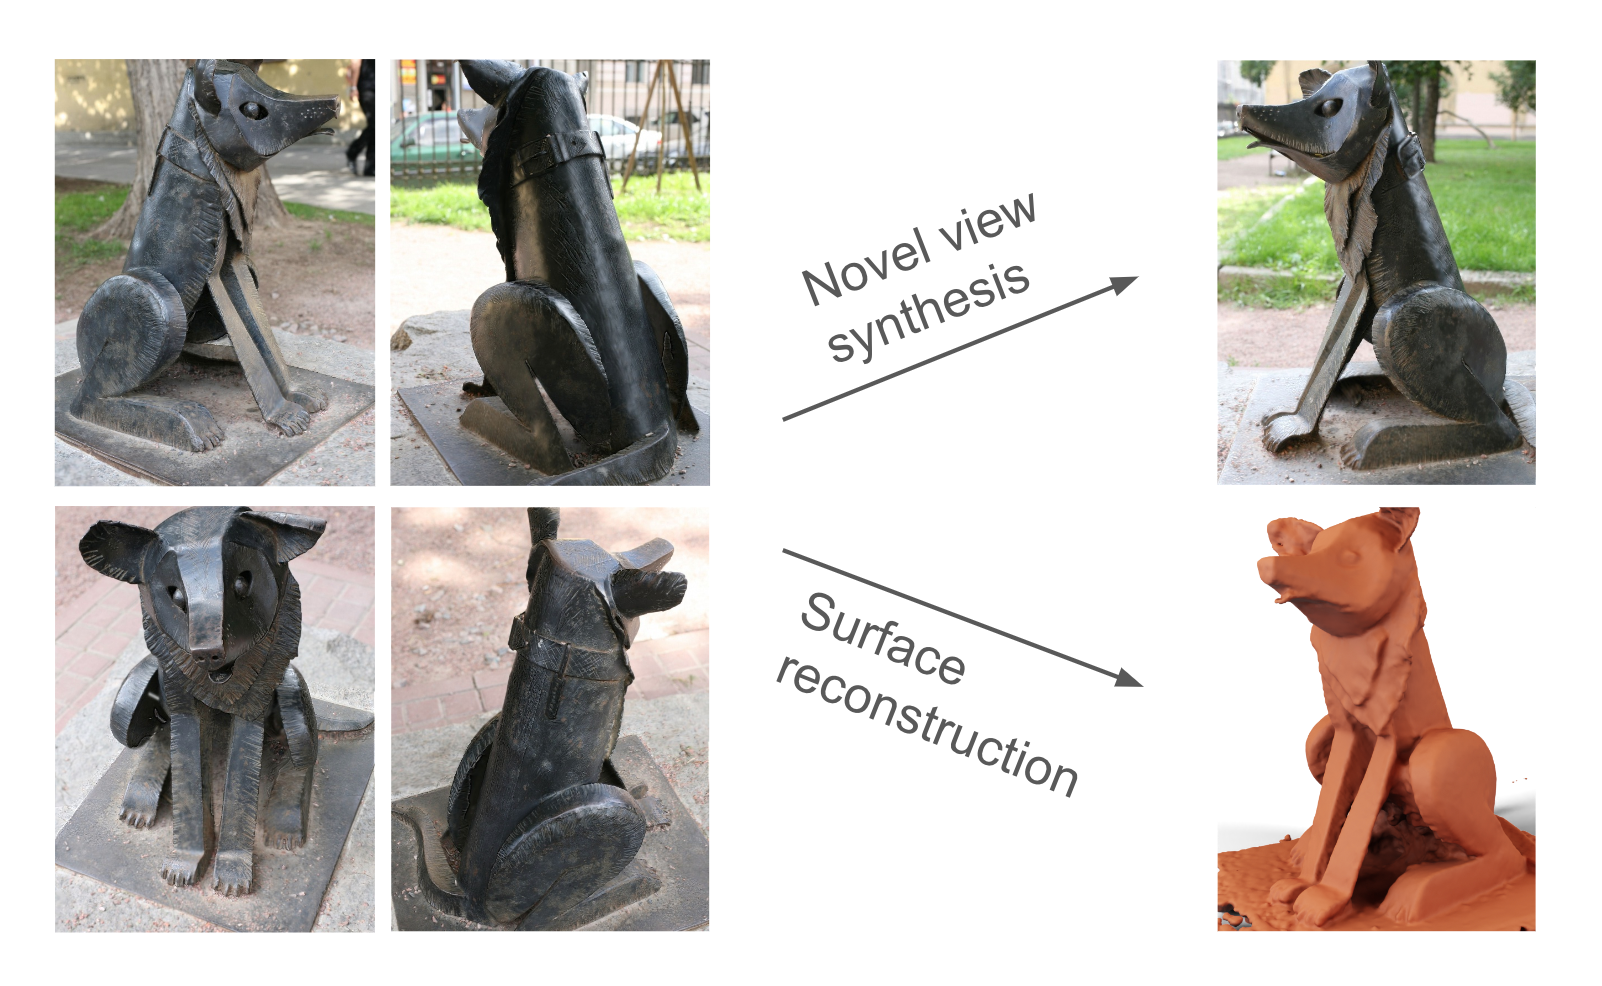
\includegraphics[width=\linewidth]{figures/intro/3d_recon.png}
        \caption{Dog scene from the Blended MVS dataset}
    \end{figure}
\end{frame}

{
\setbeamertemplate{frame footer}{\citet{berkeley_slides}}
\begin{frame}{Traditional Methods}
    \begin{itemize}
        \item Structure from motion
        \begin{figure}
            \centering
            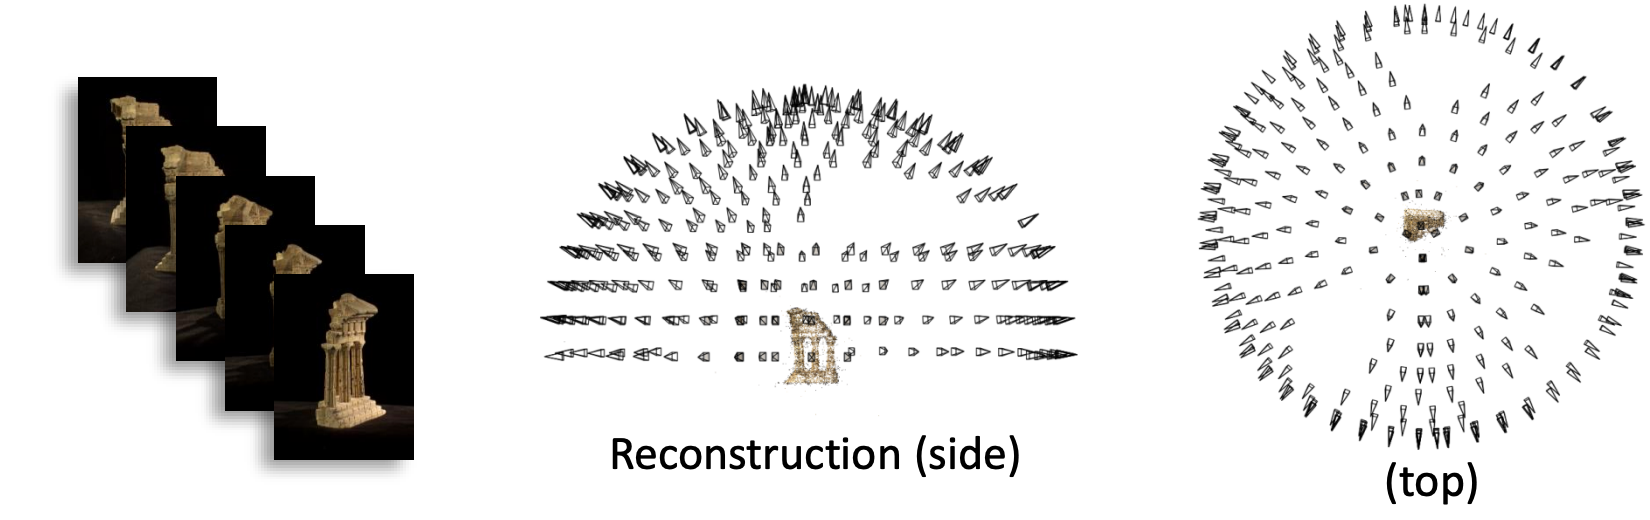
\includegraphics[width=0.7\linewidth]{figures/intro/sfm.png}
        \end{figure}
        \item Multi-view stereo
        \begin{figure}
            \centering
            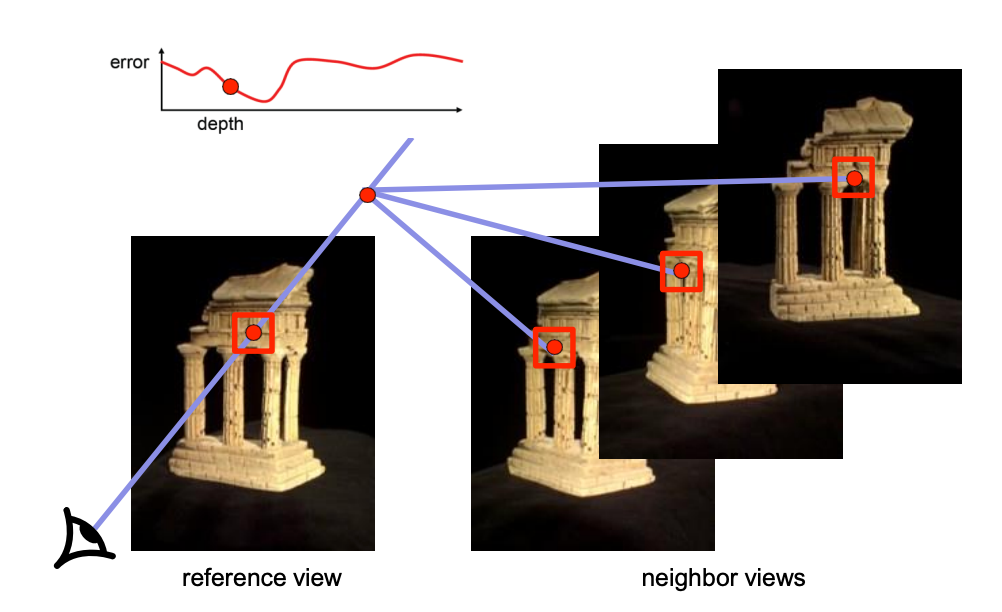
\includegraphics[width=0.6\linewidth]{figures/intro/mvs.png}
        \end{figure}
    \end{itemize}
\end{frame}
}


\begin{frame}{Traditional Methods}
    What do the outputs look like?
    
    \begin{figure}
        \centering
        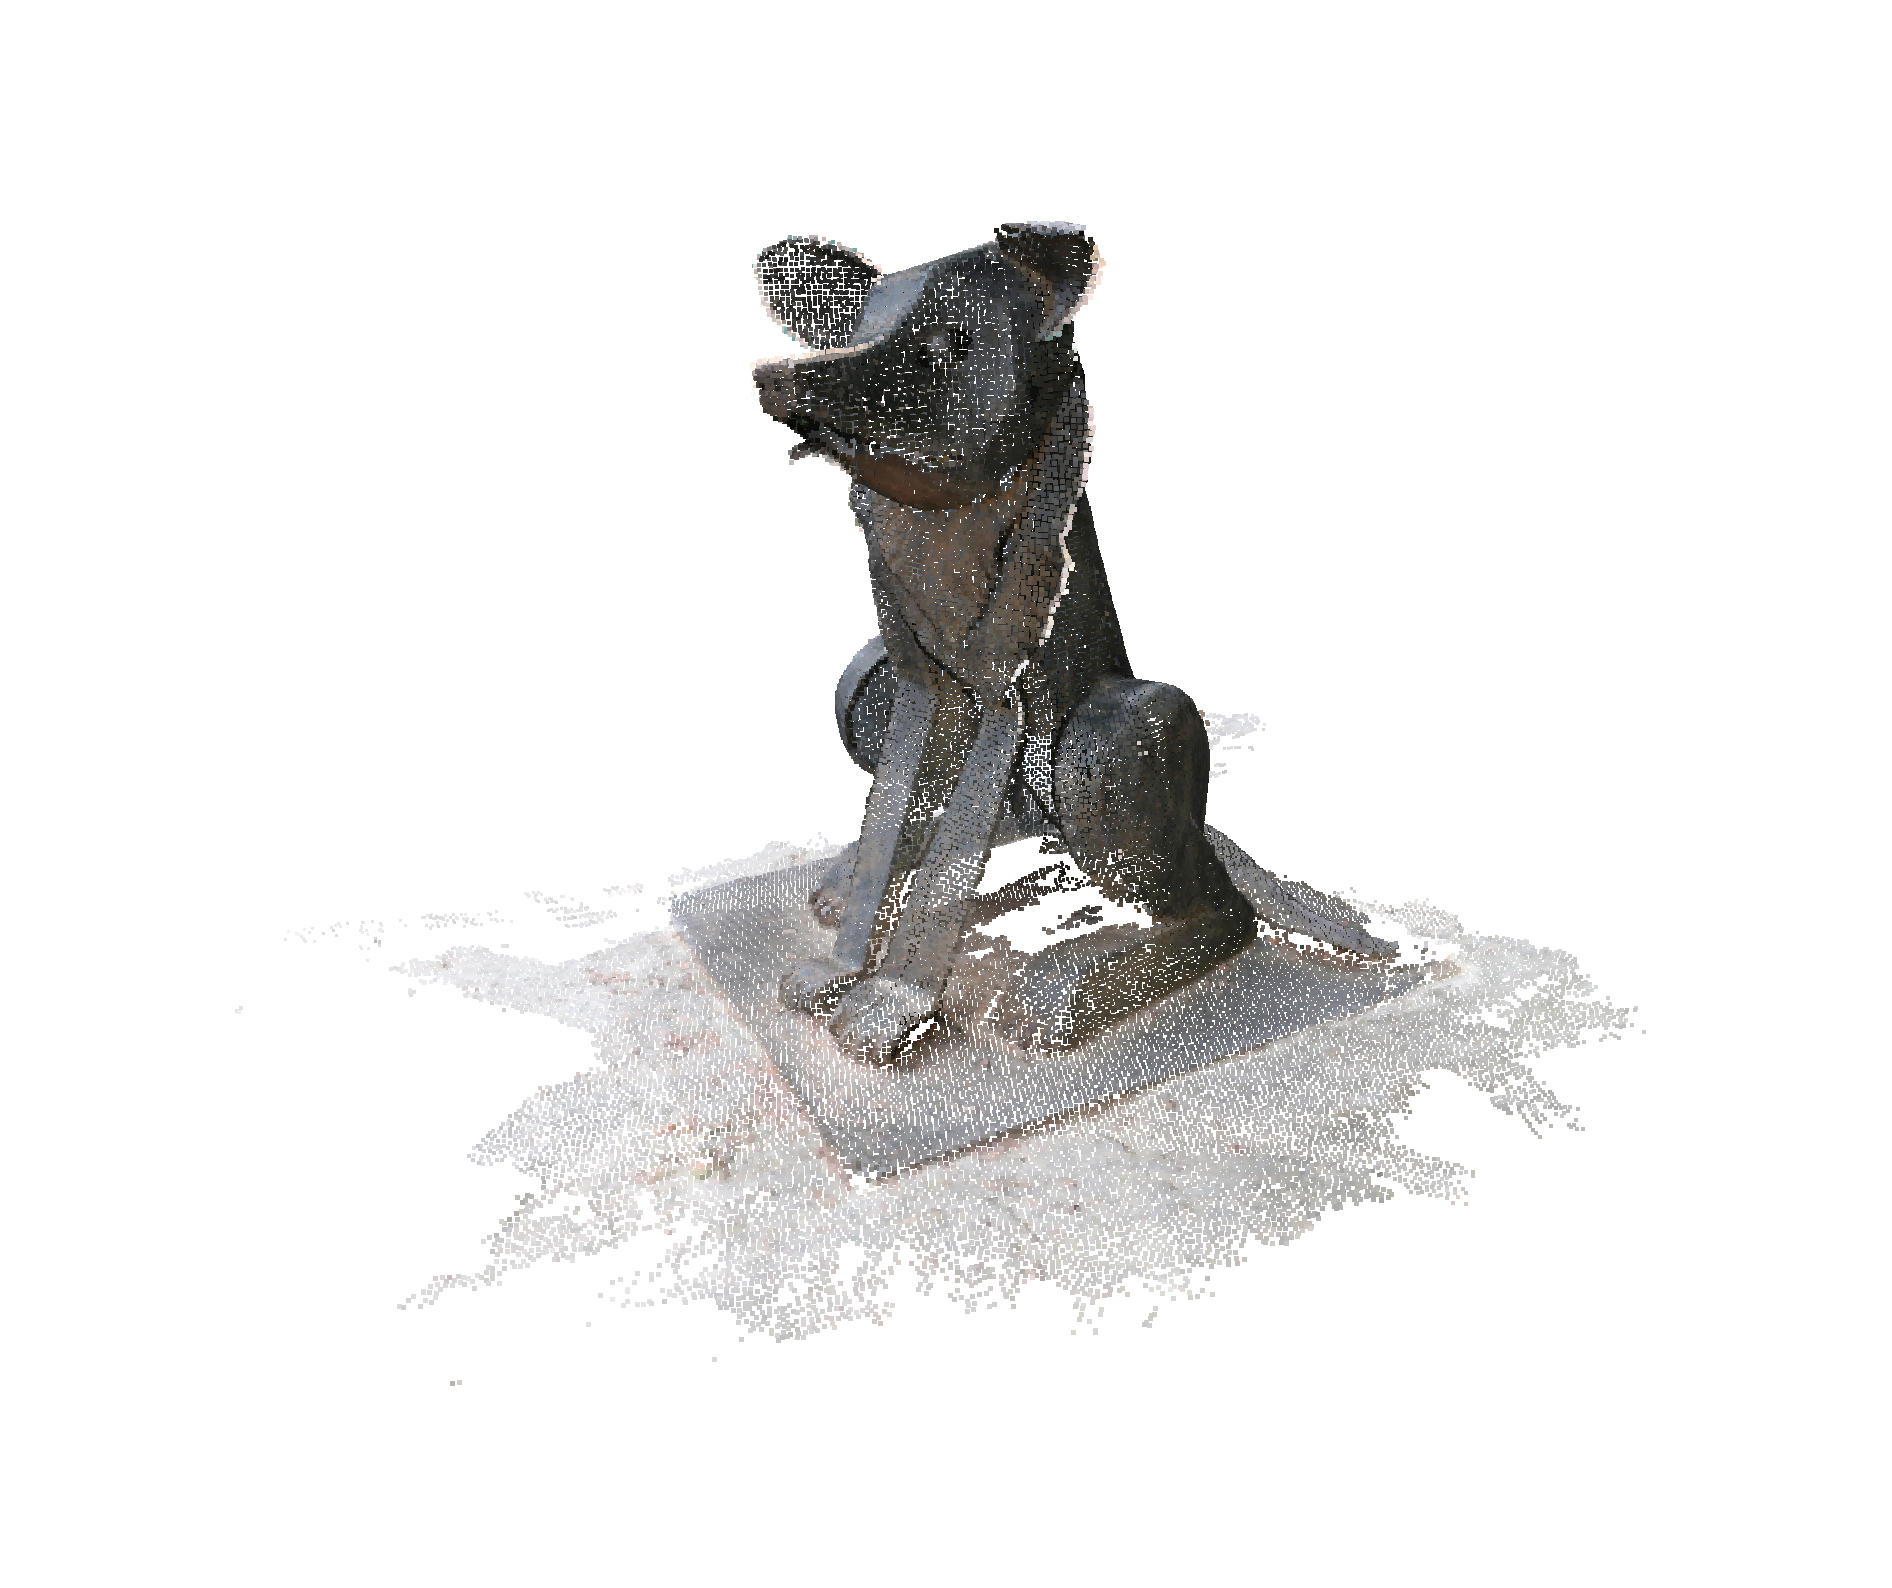
\includegraphics[width=0.8\linewidth]{figures/intro/point_cloud.png}
    \end{figure}
\end{frame}

\begin{frame}{Traditional Methods}
    Looks pretty good, except...
    
    \begin{figure}
        \centering
        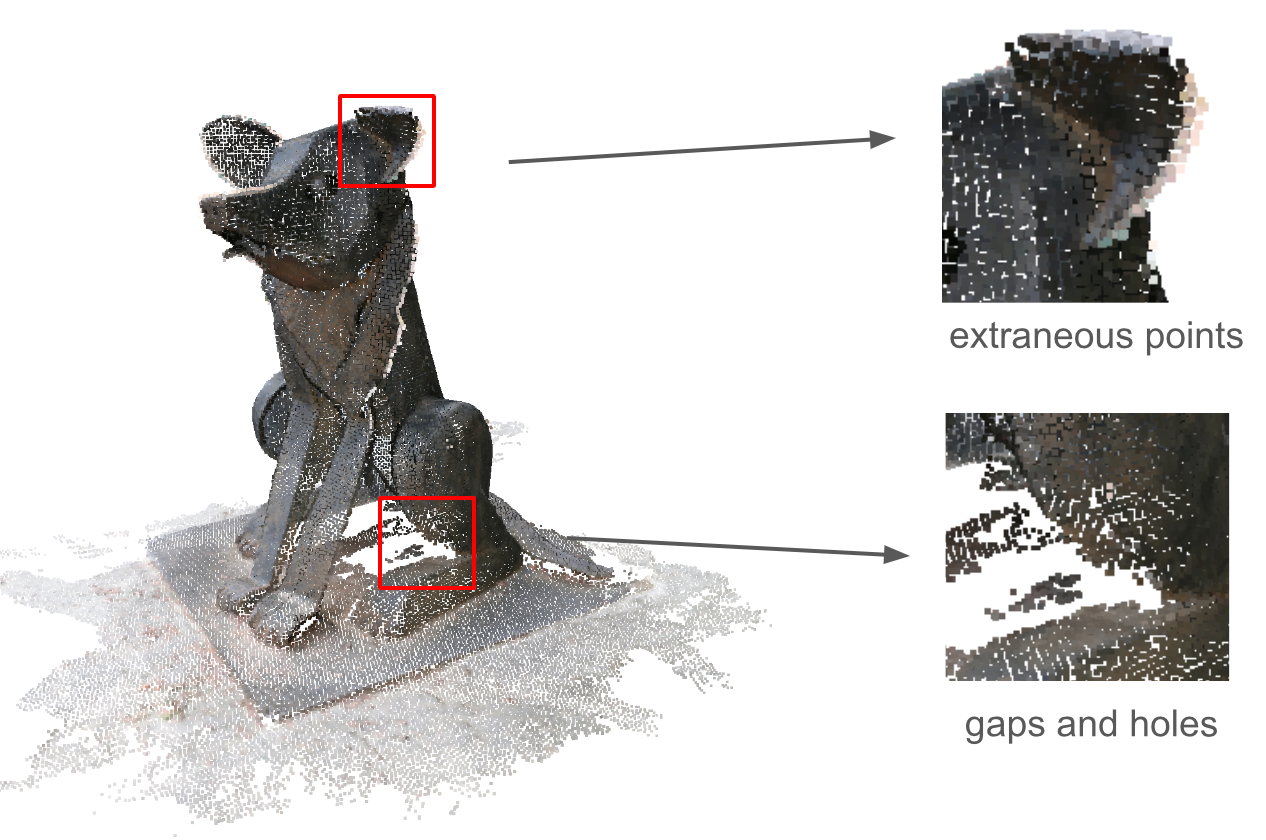
\includegraphics[width=0.8\linewidth]{figures/intro/issues.png}
    \end{figure}
\end{frame}

\begin{frame}{Traditional Methods}
    Typically, \alert{Poisson surface reconstruction} \citep{kazhdan2006poisson} is used to extract surfaces.
    
    \begin{figure}
        \centering
        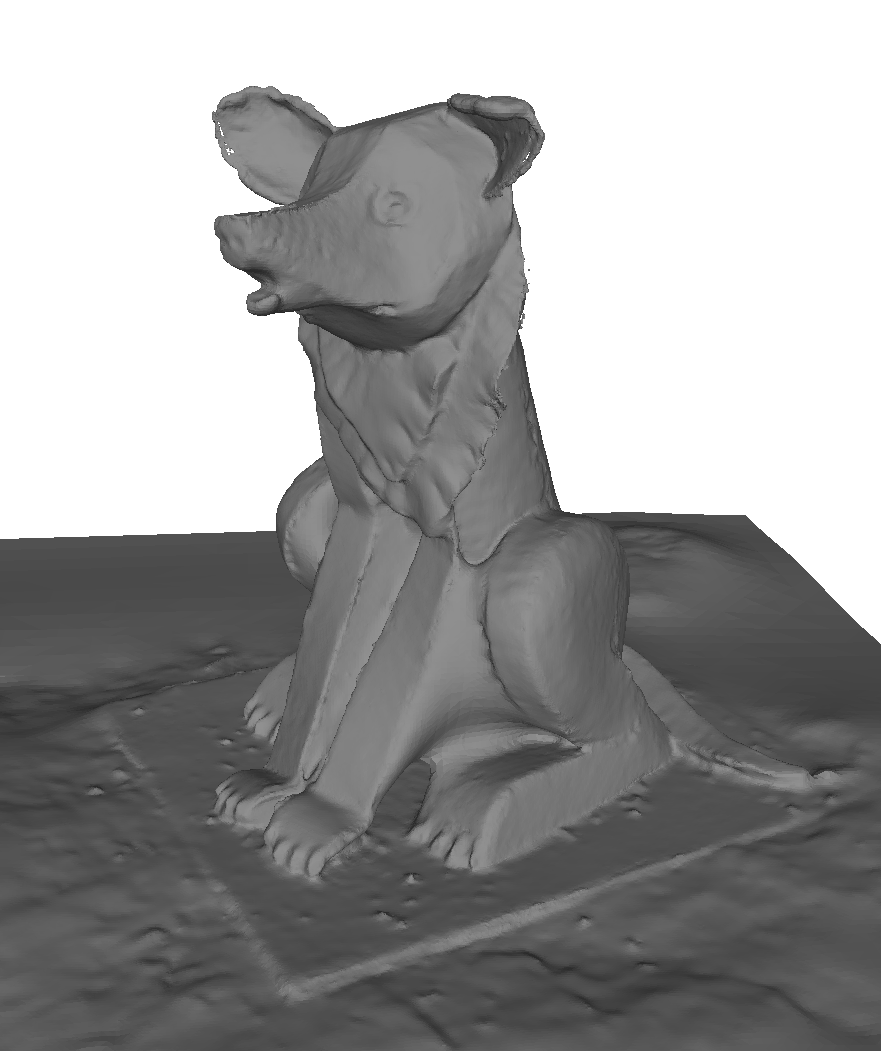
\includegraphics[width=0.5\linewidth]{figures/intro/psr.png}
    \end{figure}
\end{frame}

\begin{frame}{Traditional Methods}  
    ... and we see the same issues
    \begin{figure}
        \centering
        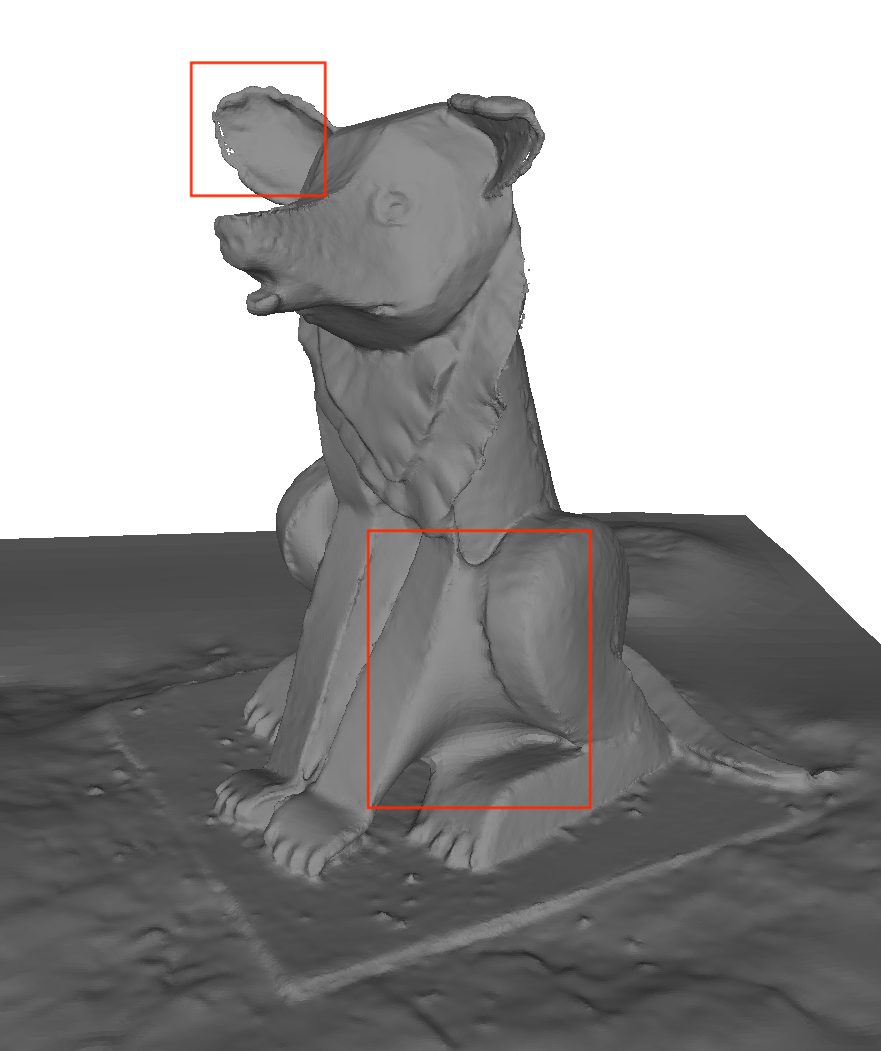
\includegraphics[width=0.5\linewidth]{figures/intro/psr_issues.png}
    \end{figure}
\end{frame}

\section{Neural Volume Rendering}

{
\setbeamertemplate{frame footer}{\citet{bunny_mesh, Park_2019_CVPR}}
\begin{frame}{Surface Rendering}
    \begin{figure}
        \centering
        \subfloat[Triangle mesh]{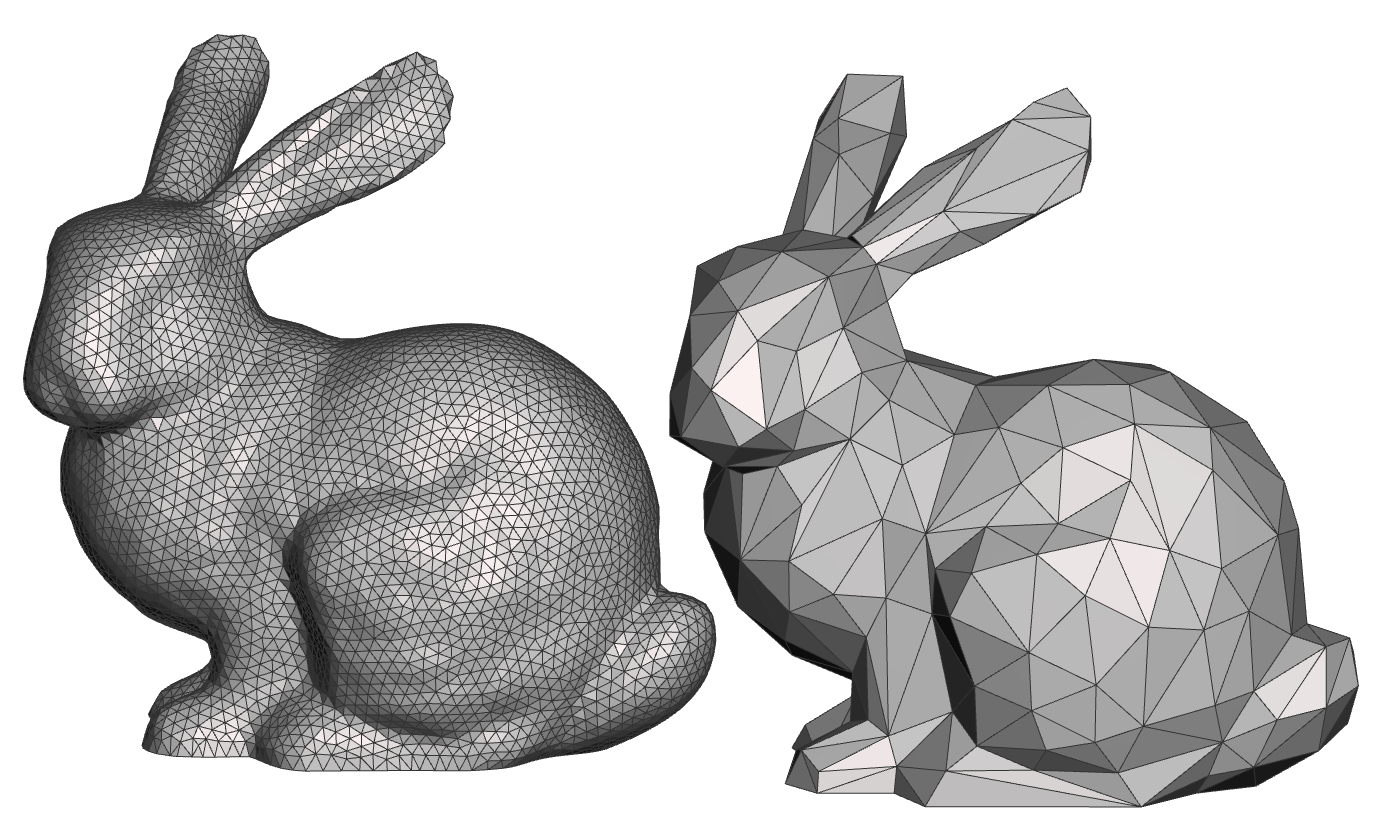
\includegraphics[width=0.45\linewidth]{figures/vol/mesh.png}}\hspace{3em}
        \subfloat[Signed-distance function]{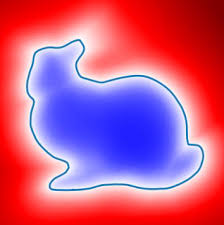
\includegraphics[width=0.35\linewidth]{figures/vol/sdf.jpg}}
    \end{figure}
\end{frame}
}

{
\setbeamertemplate{frame footer}{\citet{bitterli18framework, rte}}
\begin{frame}{Volume Rendering}
    \begin{figure}
        \centering
        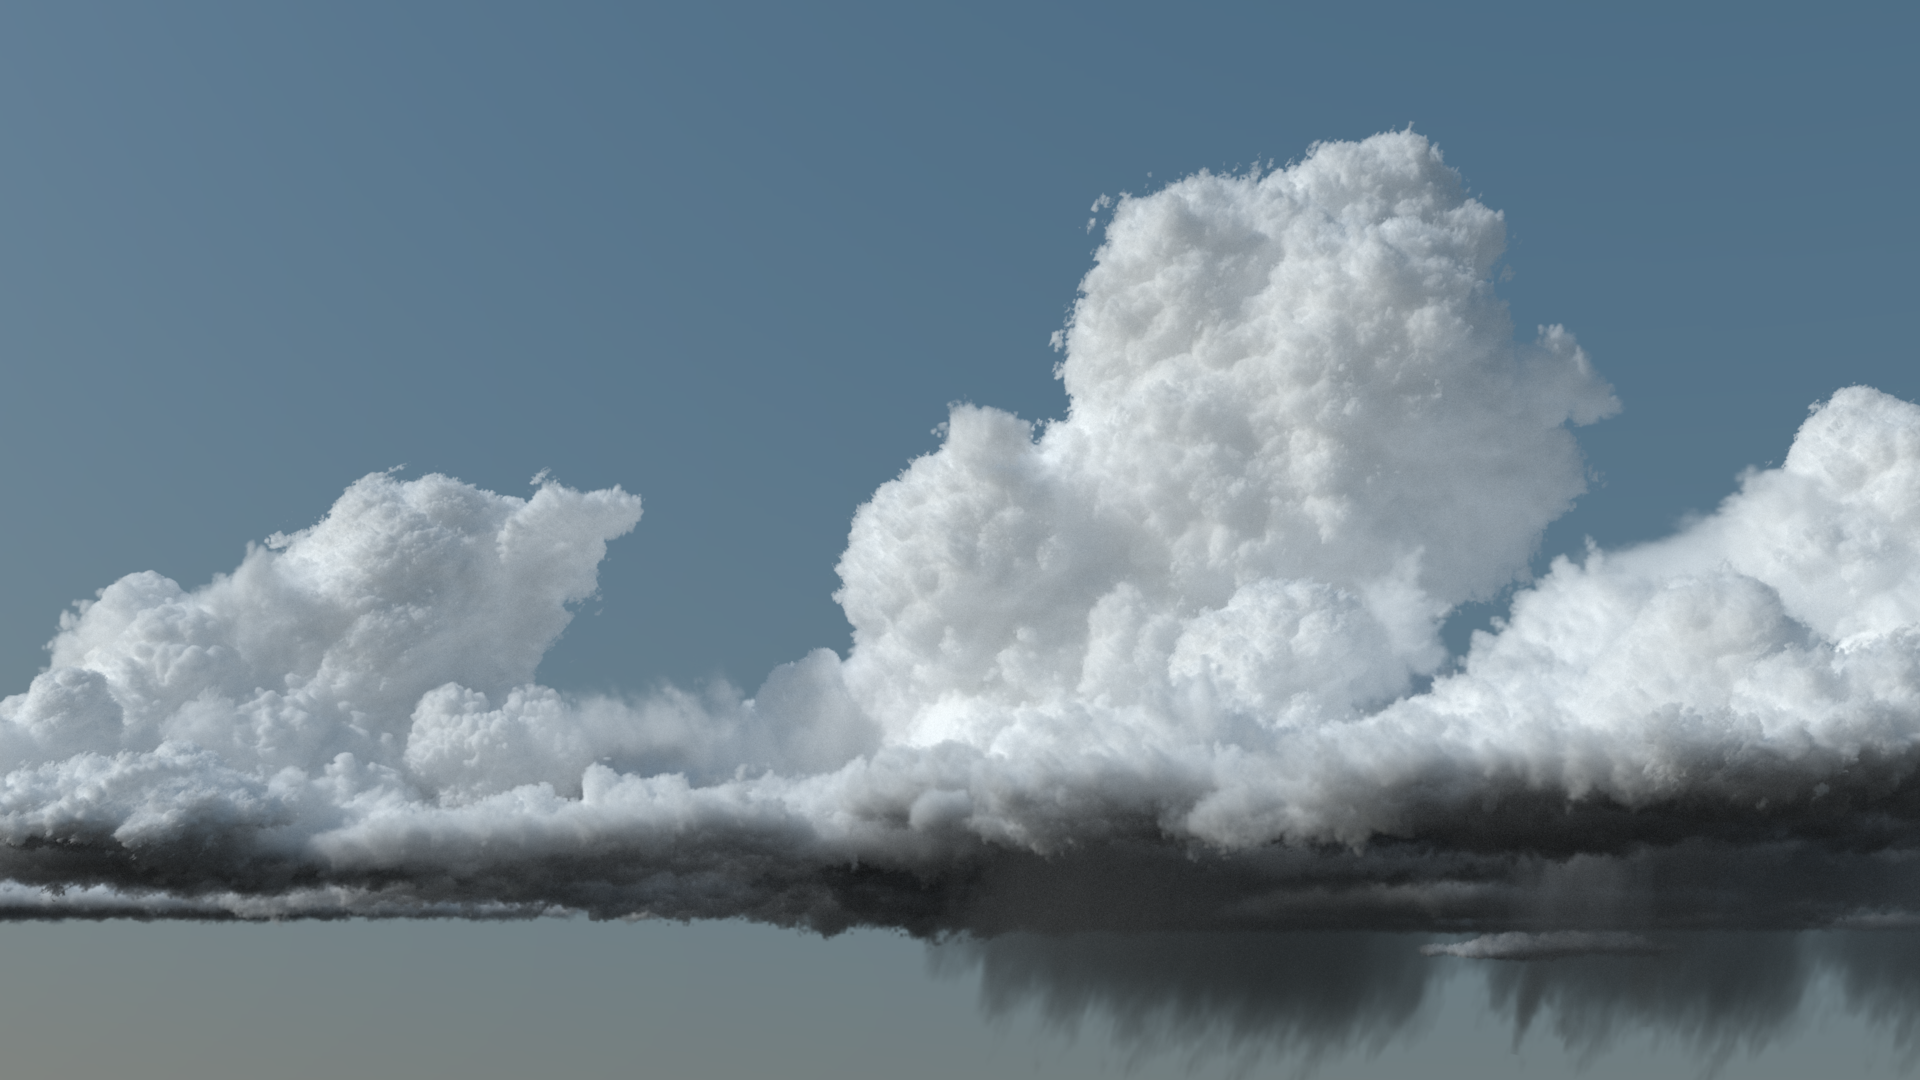
\includegraphics[width=0.6\linewidth]{figures/vol/volume.png} \\ \vspace{0.5em}
        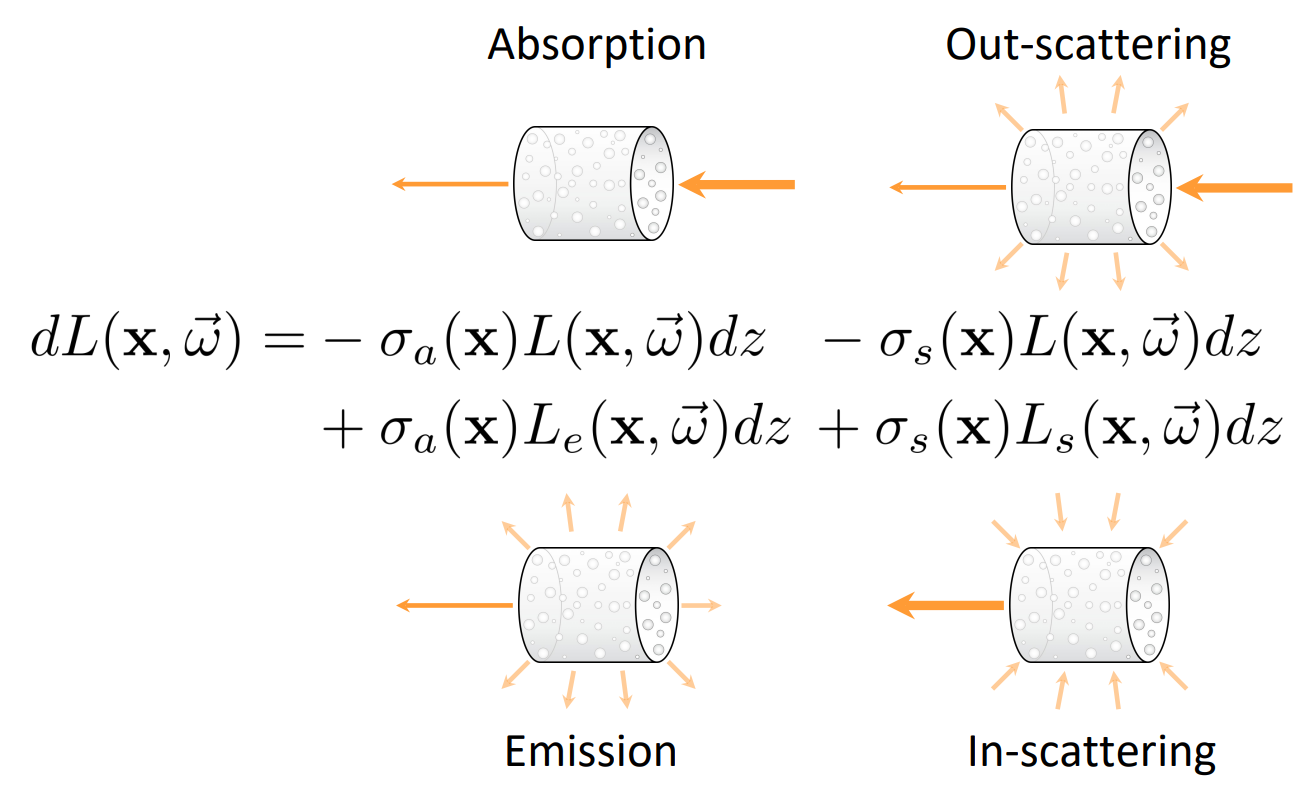
\includegraphics[width=0.5\linewidth]{figures/vol/rte.png}
    \end{figure}
\end{frame}
}

\begin{frame}{Rendering Equation}
    Assuming an \emph{emissive} volume with no scattering, we can derive the \alert{rendering equation} as
    \begin{equation*}
        L(\bx, \vec{\omega}) = \int_0^z \mathrm{Tr}(\bx, \bx_t) \sigma(\bx_t, \vec{\omega}) L_e(\bx_t, \vec{\omega})  \; \mathrm{d}t,
    \end{equation*}
    where \(\mathrm{Tr}(\bx, \bx_t)\) is the \alert{transmittance}
    \begin{equation*}
        \mathrm{Tr}(\bx, \bx_t) = \exp\left(-\int_0^t \sigma(\bx_s, \vec{\omega}) \;\mathrm{d}s\right),
    \end{equation*}
    and \(\sigma(\bx_s, \vec{\omega})\) is the spatially varying \alert{attenuation coefficient}.
\end{frame}

{
\setbeamertemplate{frame footer}{\citep{mildenhall2020nerf}}
\begin{frame}{Neural Radiance Fields (NeRF)}
    Representing objects as volumes (instead of surfaces).
    \begin{figure}
        \centering
        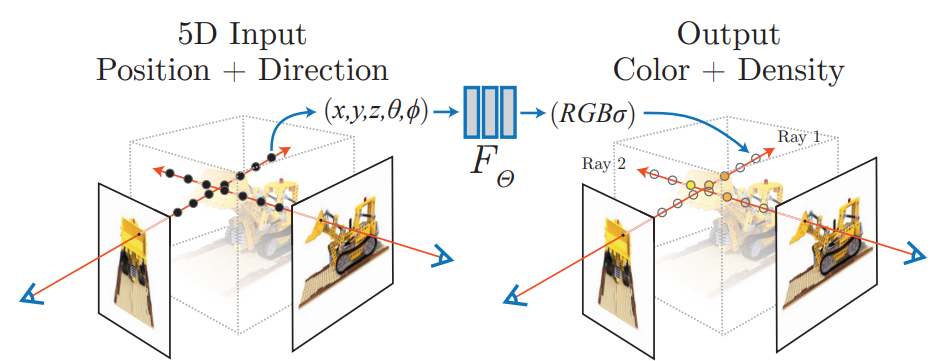
\includegraphics[width=0.9\linewidth]{figures/vol/nerf.png}
    \end{figure}

    Color \(L_e(x, \vec{\omega})\) and density \(\sigma(x, \vec{\omega})\) modeled by a \alert{neural network}.
\end{frame}

\begin{frame}{Neural Radiance Fields (NeRF)}
    NeRFs work particularly well for \alert{novel-view synthesis} tasks \\

    ... but not so much for \alert{surface extraction}.

    \begin{figure}
        \centering
        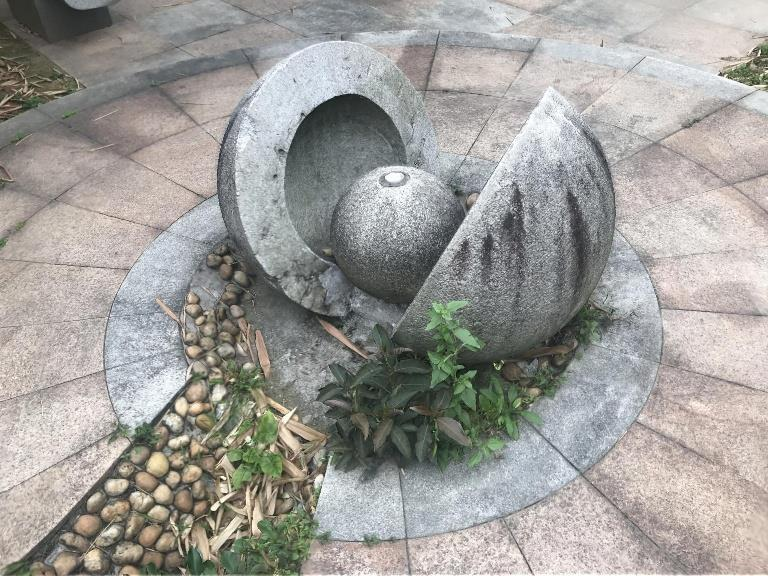
\includegraphics[width=0.35\linewidth]{figures/vol/nerf_surface/143.jpg}
        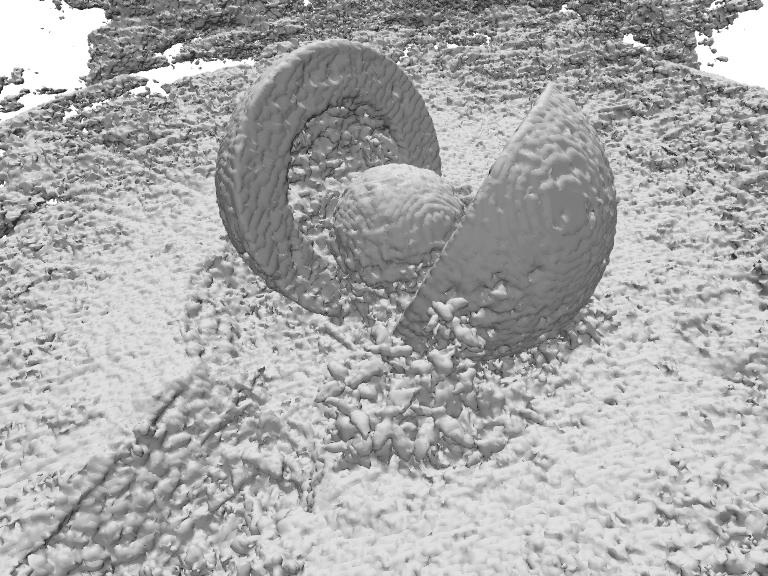
\includegraphics[width=0.35\linewidth]{figures/vol/nerf_surface/1.png} \\ \vspace{0.1em}
        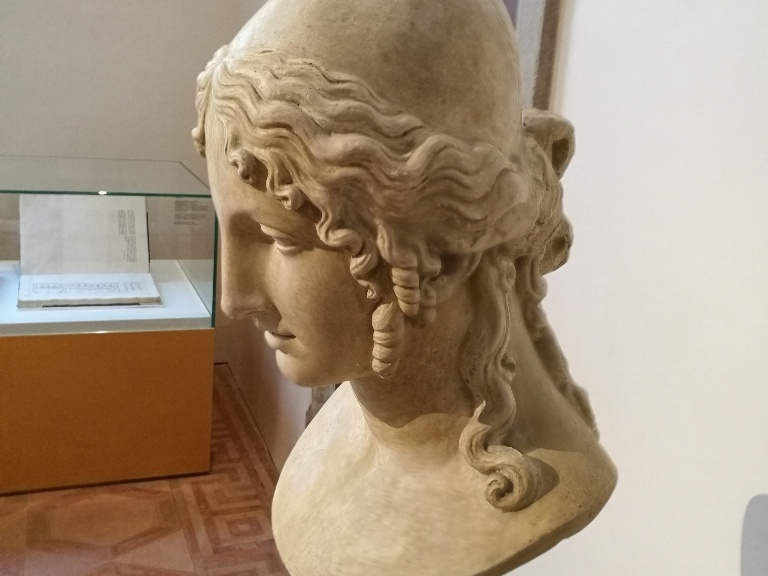
\includegraphics[width=0.35\linewidth]{figures/vol/nerf_surface/32.jpg}
        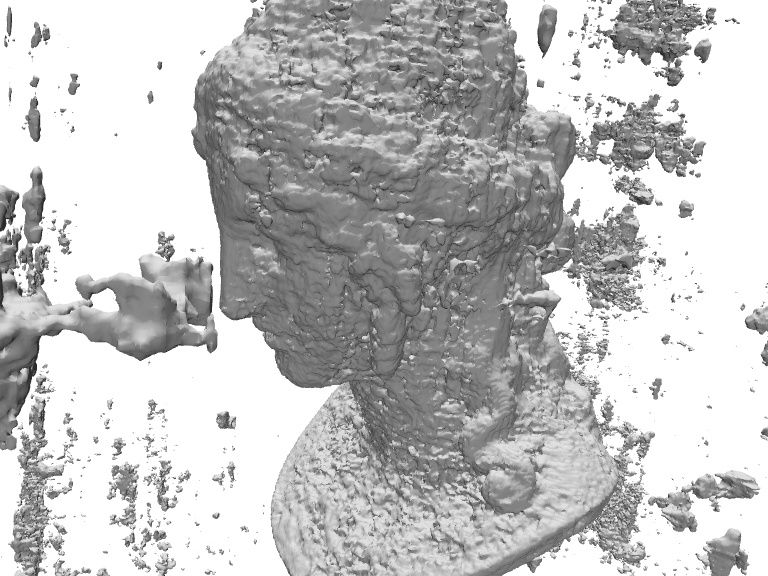
\includegraphics[width=0.35\linewidth]{figures/vol/nerf_surface/2.png}
    \end{figure}
\end{frame}
}

\begin{frame}{Neural Surface Representations}
    Can we explicitly model the \alert{geometry} of the scene?

    Yes, there are many works that already do this:
    \begin{itemize}
        \item Occupancy \(\leftrightarrow\) density {\tiny (NeuS \citep{wang2021neus})}
        \item Signed-distance function \(\leftrightarrow\) density {\tiny (VolSDF \citep{yariv2021volume})}
    \end{itemize}

    Follow-up works improve reconstruction quality and efficiency:
    \begin{itemize}
        \item Multi-resolution hash grids {\tiny (Neuralangelo \citep{li2023neuralangelo}, NeuS2 \citep{neus2})}
        \item Photo-consistency constraints {\tiny (Neuralwarp \citep{neuralwarp}, Geo-NeuS \citep{Fu2022GeoNeus})}
        \item Sparse voxel representation {\tiny (Voxurf \citep{wu2022voxurf})}
    \end{itemize}
\end{frame}

\begin{frame}{Neural Surface Representations}
    Limitations of existing methods:
    \begin{itemize}
        \item Trade-off between speed and reconstruction quality
        \item Cannot effectively leverage \alert{known information}
    \end{itemize}

    Our solution: Directly build off of the output of traditional methods (i.e. dense \alert{point clouds})
\end{frame}

\section{Winding Number \& Dipole Sums}

{
\setbeamertemplate{frame footer}{\citet{wn,Barill:FW:2018}}
\begin{frame}{The Winding Number}
    \begin{figure}
        \centering
        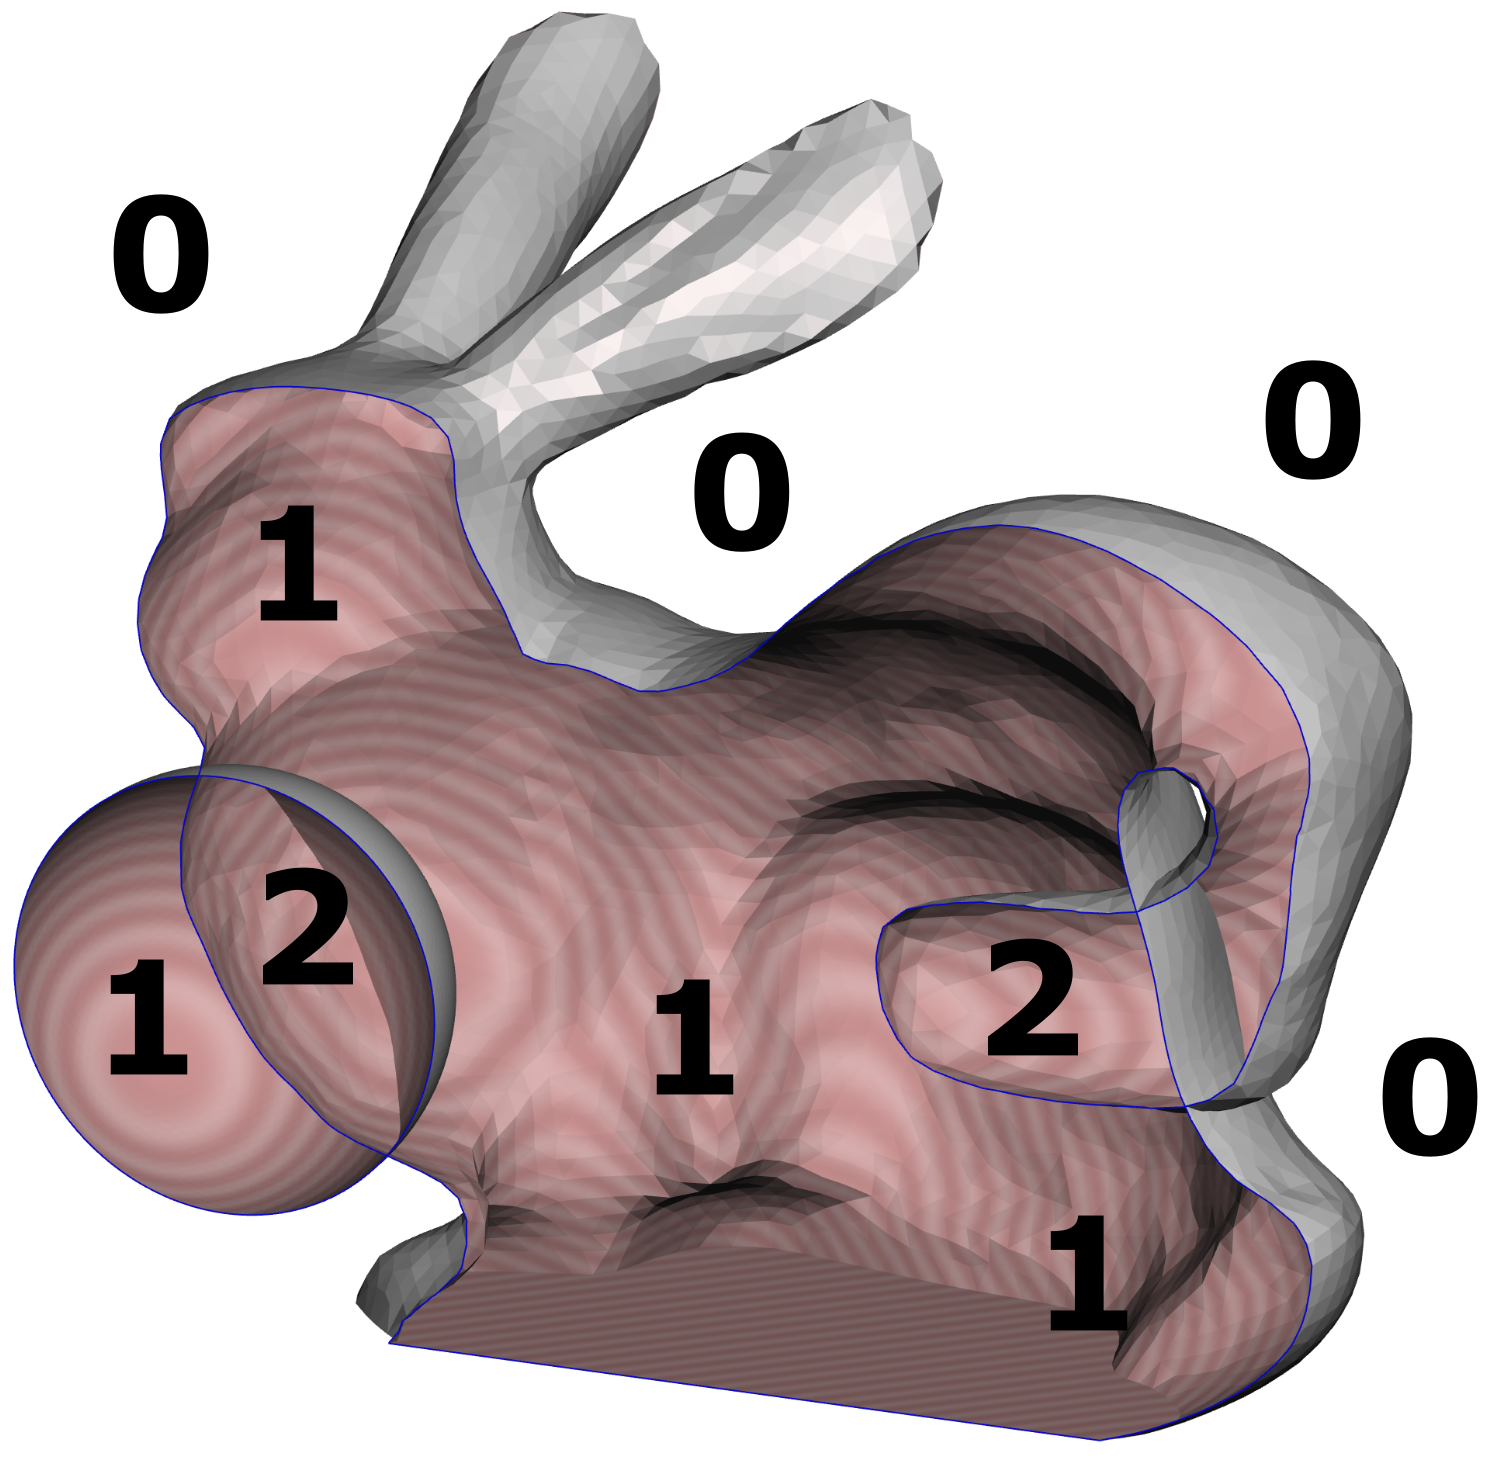
\includegraphics[width=0.4\linewidth]{figures/wn/wn.png}
    \end{figure}
    
    \begin{equation*}
        w_S(\bq) = \frac{1}{4\pi} \int_{S} \mathrm{d}\Omega(\bq) = \int_{S} \frac{(\bp - \bq) \cdot \widehat{\bn}}{4\pi \|\bp - \bq\|^3} \; \mathrm{d}\bp
    \end{equation*}
\end{frame}
}

{
\setbeamertemplate{frame footer}{\citet{Barill:FW:2018}}
\begin{frame}{The \alert{Generalized} Winding Number}
    \begin{figure}
        \centering
        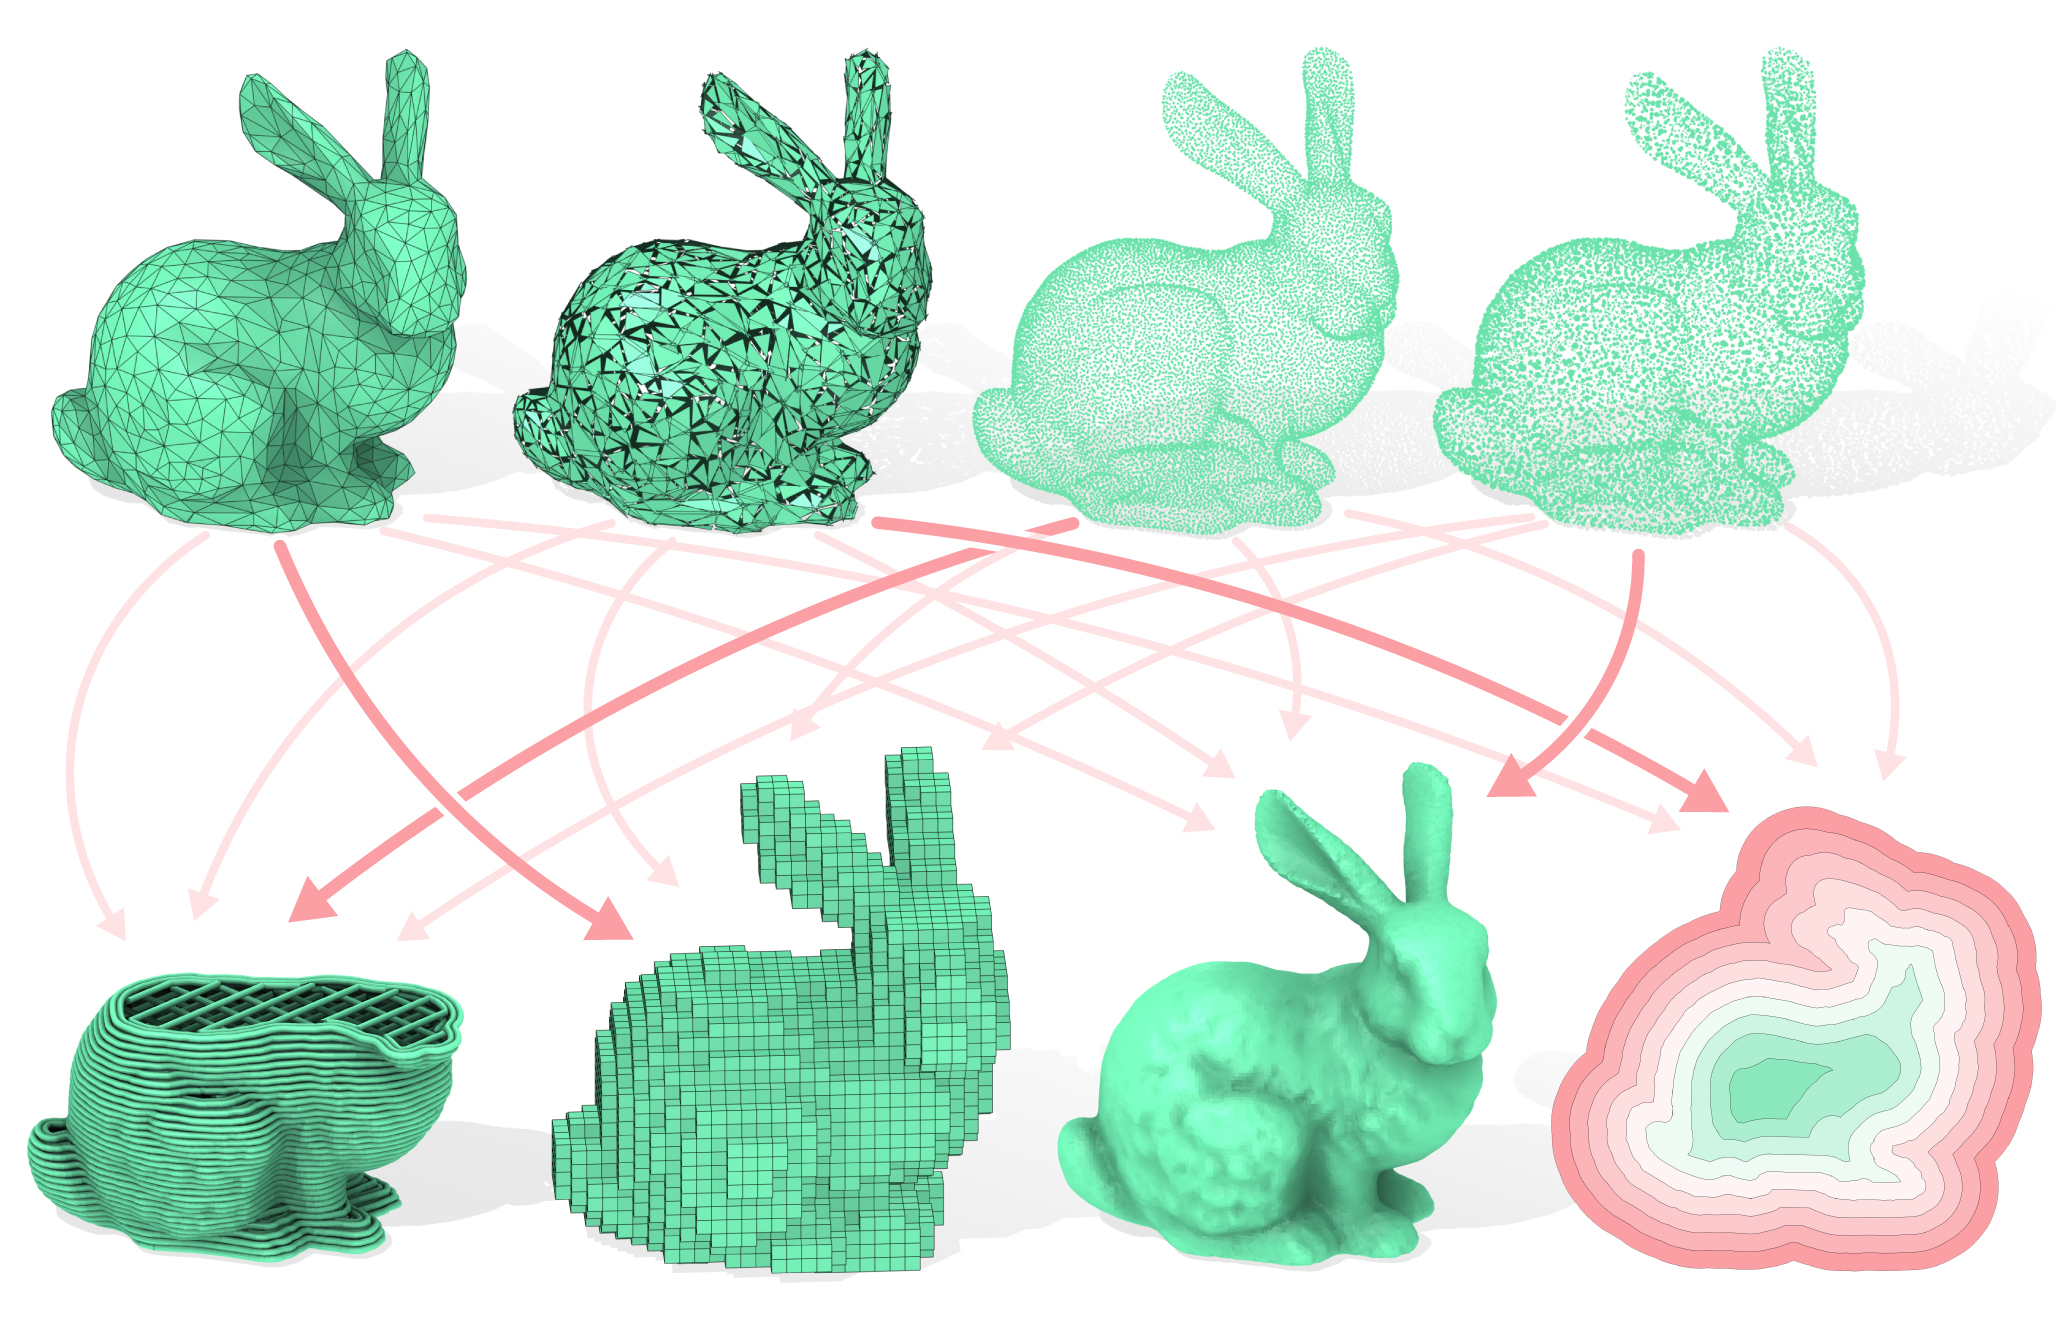
\includegraphics[width=0.6\linewidth]{figures/wn/gwn.png}
    \end{figure}

    For point clouds,
    \begin{equation*}
        w_S(\bq) \approx \sum_{m=1}^{N} a_m \frac{(\bp_m - \bq)\cdot \widehat{\bn}_m}{4\pi\|\bp_m - \bq\|^3}
    \end{equation*}
    where \(a_m\) are ``area-weights'' (e.g. geodesic Voronoi area).
\end{frame}
}

\begin{frame}{\alert{Aside}: Laplace BVP}
    The winding numbers are also the solutions to the Laplace boundary value problem (BVP)
    \begin{align*}
    \begin{cases}
        \Delta w(\bp) = 0, & \bp \in {\mathbb R}^3 \backslash \partial \Omega \\
        w^+(\bp) - w^-(\bp) = f(\bp), & \bp \in \partial \Omega \\
        \frac{\partial w^+}{\partial \widehat{\bn}}(\bp) - \frac{\partial w^-}{\partial \widehat{\bn}}(\bp) = 0, & \bp \in  \partial \Omega,
    \end{cases}
    \end{align*}
    for the specific case where \(f(\bp) \equiv 1\) on the boundary.
\end{frame}

\begin{frame}{The \alert{Generalized} Winding Number}
    Naively, we can directly extract the \(0.5\)-isosurface of the winding number field. However, this often fails in practice...
    \vspace{-1em}
    \begin{figure}
        \centering
        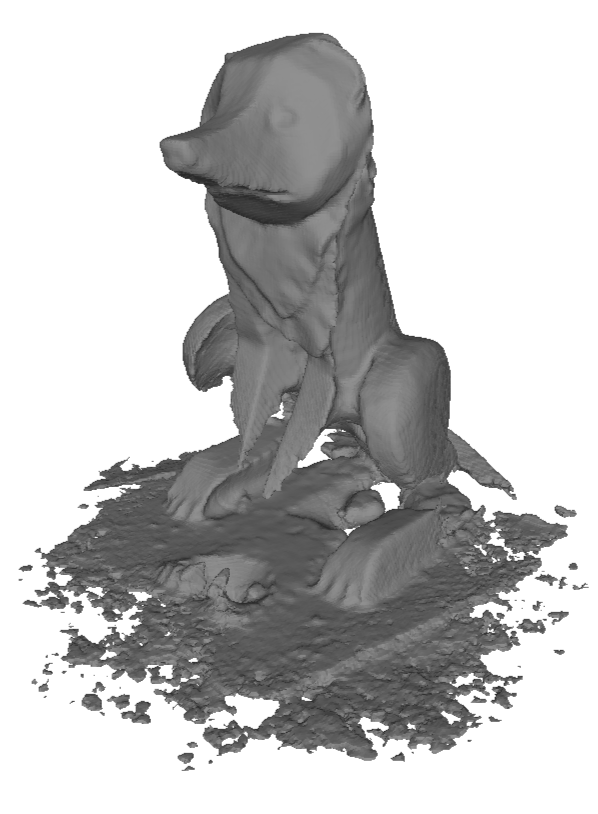
\includegraphics[width=0.45\linewidth]{figures/wn/gwn_mesh.png}
    \end{figure}
\end{frame}

\begin{frame}{The Dipole Sum}
    What if we further generalize the winding number
    
    ... and allow \(f(\bp) \not\equiv 1\)?
    \begin{align*}
        w_S(\bq) = \int_{S} &\frac{(\bp - \bq) \cdot \widehat{\bn}}{4\pi \|\bp - \bq\|^3} \cdot 1 \;\mathrm{d}\bp \\
        &\Downarrow \\
        u^f_S(\bq) = \int_{S} & \frac{(\bp - \bq) \cdot \widehat{\bn}}{4\pi \|\bp - \bq\|^3} \cdot f(\bp) \;\mathrm{d}\bp
    \end{align*}
\end{frame}

\begin{frame}{The Dipole Sum}
    This is equivalent to having non-unit \alert{per-point} attributes \(f_m\):
    \begin{align*}
        w_{\mathrm{pc}}(\bq) = \sum_{m=1}^{N} &a_m \frac{(\bp_m - \bq)\cdot \widehat{\bn}_m}{4\pi\|\bp_m - \bq\|^3} \cdot 1 \\
        &\Downarrow \\
        u^f_{\mathrm{pc}}(\bq) = \sum_{m=1}^{N} &a_m \frac{(\bp_m - \bq) \cdot \widehat{\bn}_m}{4\pi \|\bp_m - \bq\|^3} \cdot f_m
    \end{align*}

    In a differentiable rendering pipeline, we can make them learnable!
\end{frame}

\begin{frame}{The \alert{Fast} Dipole Sum}
    A dense point cloud can have tens of thousands of points
    
    ... and to render a single image, we need to potentially query the dipole sum at billions of distinct locations in the scene.

    Obviously, we cannot compute the entire sum for every query...
\end{frame}

\begin{frame}{The Barne-Hut Approximation}
    As proposed by \citet{Barill:FW:2018}, we can consider a cluster of points far away from the query point as a single ``dipole'' with attributes computed using the \alert{Barnes-Hut approximation}.

    \begin{figure}
        \centering
        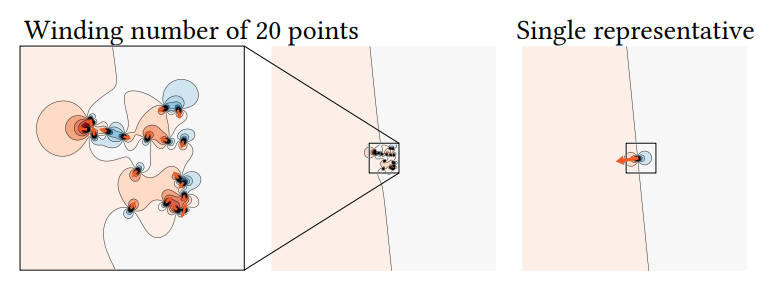
\includegraphics[width=0.9\linewidth]{figures/wn/barne_hut.png}
    \end{figure}
\end{frame}

\begin{frame}{The Barne-Hut Approximation}
    We construct an \alert{octree} from the point cloud, and assign each tree node \(t\) a centroid, a weighted normal, and a radius, computed from its leaves \(\mathcal L(t)\):
    \begin{align*}
        \tilde{\bp}_t & \equiv \frac{\sum_{m \in \mathcal L(t)} a_m \bp_m}{\sum_{m \in \mathcal L(t)} a_m} \\
        \tilde{\bn}^f_t & \equiv \sum_{m \in \mathcal L(t)} a_m \widehat{\bn}_m \cdot f_m \\
        \tilde{r}_t & \equiv \max_{m \in \mathcal L(t)} \|\tilde{\bp}_t - \bp_m\|
    \end{align*}

    To query the \alert{fast} dipole sum, we recurse the octree with aggressive pruning in \(O(\log N)\) time.
\end{frame}

\begin{frame}[standout]
  Questions?
\end{frame}

% \appendix

\begin{frame}[allowframebreaks]{References}

  \bibliography{ref}
  \bibliographystyle{plainnat}

\end{frame}

\end{document}
